%%%%%%%%%%%%%%%%%%%%%%%%%%%%%%%%%%%%%%%%%
% 
% MDM Poster Template
%
%%%%%%%%%%%%%%%%%%%%%%%%%%%%%%%%%%%%%%%%%

%----------------------------------------------------------------------------------------
%	PACKAGES AND OTHER DOCUMENT CONFIGURATIONS
%----------------------------------------------------------------------------------------

\documentclass[a0,landscape]{a0poster}

% Macros for Fitch-style natural deduction. 
% Author: Peter Selinger, University of Ottawa
% Created: Jan 14, 2002
% Modified: Feb 8, 2005
% Version: 0.5
% Copyright: (C) 2002-2005 Peter Selinger
% Filename: fitch.sty
% Documentation: fitchdoc.tex
% URL: http://quasar.mathstat.uottawa.ca/~selinger/fitch/

% License:
%
% This program is free software; you can redistribute it and/or modify
% it under the terms of the GNU General Public License as published by
% the Free Software Foundation; either version 2, or (at your option)
% any later version.
%
% This program is distributed in the hope that it will be useful, but
% WITHOUT ANY WARRANTY; without even the implied warranty of
% MERCHANTABILITY or FITNESS FOR A PARTICULAR PURPOSE. See the GNU
% General Public License for more details.
%
% You should have received a copy of the GNU General Public License
% along with this program; if not, write to the Free Software Foundation, 
% Inc., 59 Temple Place, Suite 330, Boston, MA 02111-1307, USA.

% USAGE EXAMPLE:
% 
% The following is a simple example illustrating the usage of this
% package.  For detailed instructions and additional functionality, see
% the user guide, which can be found in the file fitchdoc.tex.
% 
% \[
% \begin{nd}
%   \hypo{1}  {P\vee Q}   
%   \hypo{2}  {\neg Q}                         
%   \open                              
%   \hypo{3a} {P}
%   \have{3b} {P}        \r{3a}
%   \close                   
%   \open
%   \hypo{4a} {Q}
%   \have{4b} {\neg Q}   \r{2}
%   \have{4c} {\bot}     \ne{4a,4b}
%   \have{4d} {P}        \be{4c}
%   \close                             
%   \have{5}  {P}        \oe{1,3a-3b,4a-4d}                 
% \end{nd}
% \]

{\chardef\x=\catcode`\*
\catcode`\*=11
\global\let\nd*astcode\x}
\catcode`\*=11

% References

\newcount\nd*ctr
\def\nd*render{\expandafter\ifx\expandafter\nd*x\nd*base\nd*x\the\nd*ctr\else\nd*base\ifnum\nd*ctr<0\the\nd*ctr\else\ifnum\nd*ctr>0+\the\nd*ctr\fi\fi\fi}
\expandafter\def\csname nd*-\endcsname{}

\def\nd*num#1{\nd*numo{\nd*render}{#1}\global\advance\nd*ctr1}
\def\nd*numopt#1#2{\nd*numo{$#1$}{#2}}
\def\nd*numo#1#2{\edef\x{#1}\mbox{$\x$}\expandafter\global\expandafter\let\csname nd*-#2\endcsname\x}
\def\nd*ref#1{\expandafter\let\expandafter\x\csname nd*-#1\endcsname\ifx\x\relax%
  \errmessage{Undefined natdeduction reference: #1}\else\mbox{$\x$}\fi}
\def\nd*noop{}
\def\nd*set#1#2{\ifx\relax#1\nd*noop\else\global\def\nd*base{#1}\fi\ifx\relax#2\relax\else\global\nd*ctr=#2\fi}
\def\nd*reset{\nd*set{}{1}}
\def\nd*refa#1{\nd*ref{#1}}
\def\nd*aux#1#2{\ifx#2-\nd*refa{#1}--\def\nd*c{\nd*aux{}}%
  \else\ifx#2,\nd*refa{#1}, \def\nd*c{\nd*aux{}}%
  \else\ifx#2;\nd*refa{#1}; \def\nd*c{\nd*aux{}}%
  \else\ifx#2.\nd*refa{#1}. \def\nd*c{\nd*aux{}}%
  \else\ifx#2)\nd*refa{#1})\def\nd*c{\nd*aux{}}%
  \else\ifx#2(\nd*refa{#1}(\def\nd*c{\nd*aux{}}%
  \else\ifx#2\nd*end\nd*refa{#1}\def\nd*c{}%
  \else\def\nd*c{\nd*aux{#1#2}}%
  \fi\fi\fi\fi\fi\fi\fi\nd*c}
\def\ndref#1{\nd*aux{}#1\nd*end}

% Layer A

% define various dimensions (explained in fitchdoc.tex):
\newlength{\nd*dim} 
\newdimen\nd*depthdim
\newdimen\nd*hsep
\newdimen\ndindent
\ndindent=1em
% user command to redefine dimensions
\def\nddim#1#2#3#4#5#6#7#8{\nd*depthdim=#3\relax\nd*hsep=#6\relax%
\def\nd*height{#1}\def\nd*thickness{#8}\def\nd*initheight{#2}%
\def\nd*indent{#5}\def\nd*labelsep{#4}\def\nd*justsep{#7}}
% set initial dimensions
\nddim{4.5ex}{3.5ex}{1.5ex}{1em}{1.6em}{.5em}{2.5em}{.2mm}

\def\nd*v{\rule[-\nd*depthdim]{\nd*thickness}{\nd*height}}
\def\nd*t{\rule[-\nd*depthdim]{0mm}{\nd*height}\rule[-\nd*depthdim]{\nd*thickness}{\nd*initheight}}
\def\nd*i{\hspace{\nd*indent}} 
\def\nd*s{\hspace{\nd*hsep}}
\def\nd*g#1{\nd*f{\makebox[\nd*indent][c]{$#1$}}}
\def\nd*f#1{\raisebox{0pt}[0pt][0pt]{$#1$}}
\def\nd*u#1{\makebox[0pt][l]{\settowidth{\nd*dim}{\nd*f{#1}}%
    \addtolength{\nd*dim}{2\nd*hsep}\hspace{-\nd*hsep}\rule[-\nd*depthdim]{\nd*dim}{\nd*thickness}}\nd*f{#1}}

% Lists

\def\nd*push#1#2{\expandafter\gdef\expandafter#1\expandafter%
  {\expandafter\nd*cons\expandafter{#1}{#2}}}
\def\nd*pop#1{{\def\nd*nil{\gdef#1{\nd*nil}}\def\nd*cons##1##2%
    {\gdef#1{##1}}#1}}
\def\nd*iter#1#2{{\def\nd*nil{}\def\nd*cons##1##2{##1#2{##2}}#1}}
\def\nd*modify#1#2#3{{\def\nd*nil{\gdef#1{\nd*nil}}\def\nd*cons##1##2%
    {\advance#2-1 ##1\advance#2 1 \ifnum#2=1\nd*push#1{#3}\else%
      \nd*push#1{##2}\fi}#1}}

\def\nd*cont#1{{\def\nd*t{\nd*v}\def\nd*v{\nd*v}\def\nd*g##1{\nd*i}%
    \def\nd*i{\nd*i}\def\nd*nil{\gdef#1{\nd*nil}}\def\nd*cons##1##2%
    {##1\expandafter\nd*push\expandafter#1\expandafter{##2}}#1}}

% Layer B

\newcount\nd*n
\def\nd*beginb{\begingroup\nd*reset\gdef\nd*stack{\nd*nil}\nd*push\nd*stack{\nd*t}%
  \begin{array}{l@{\hspace{\nd*labelsep}}l@{\hspace{\nd*justsep}}l}}
\def\nd*resumeb{\begingroup\begin{array}{l@{\hspace{\nd*labelsep}}l@{\hspace{\nd*justsep}}l}}
\def\nd*endb{\end{array}\endgroup}
\def\nd*hypob#1#2{\nd*f{\nd*num{#1}}&\nd*iter\nd*stack\relax\nd*cont\nd*stack\nd*s\nd*u{#2}&}
\def\nd*haveb#1#2{\nd*f{\nd*num{#1}}&\nd*iter\nd*stack\relax\nd*cont\nd*stack\nd*s\nd*f{#2}&}
\def\nd*havecontb#1#2{&\nd*iter\nd*stack\relax\nd*cont\nd*stack\nd*s\nd*f{\hspace{\ndindent}#2}&}
\def\nd*hypocontb#1#2{&\nd*iter\nd*stack\relax\nd*cont\nd*stack\nd*s\nd*u{\hspace{\ndindent}#2}&}

\def\nd*openb{\nd*push\nd*stack{\nd*i}\nd*push\nd*stack{\nd*t}}
\def\nd*closeb{\nd*pop\nd*stack\nd*pop\nd*stack}
\def\nd*guardb#1#2{\nd*n=#1\multiply\nd*n by 2 \nd*modify\nd*stack\nd*n{\nd*g{#2}}}

% Layer C

\def\nd*clr{\gdef\nd*cmd{}\gdef\nd*typ{\relax}}
\def\nd*sto#1#2#3{\gdef\nd*typ{#1}\gdef\nd*byt{}%
  \gdef\nd*cmd{\nd*typ{#2}{#3}\nd*byt\\}}
\def\nd*chtyp{\expandafter\ifx\nd*typ\nd*hypocontb\def\nd*typ{\nd*havecontb}\else\def\nd*typ{\nd*haveb}\fi}
\def\nd*hypoc#1#2{\nd*chtyp\nd*cmd\nd*sto{\nd*hypob}{#1}{#2}}
\def\nd*havec#1#2{\nd*cmd\nd*sto{\nd*haveb}{#1}{#2}}
\def\nd*hypocontc#1{\nd*chtyp\nd*cmd\nd*sto{\nd*hypocontb}{}{#1}}
\def\nd*havecontc#1{\nd*cmd\nd*sto{\nd*havecontb}{}{#1}}
\def\nd*by#1#2{\ifx\nd*x#2\nd*x\gdef\nd*byt{\mbox{#1}}\else\gdef\nd*byt{\mbox{#1, \ndref{#2}}}\fi}

% multi-line macros
\def\nd*mhypoc#1#2{\nd*mhypocA{#1}#2\\\nd*stop\\}
\def\nd*mhypocA#1#2\\{\nd*hypoc{#1}{#2}\nd*mhypocB}
\def\nd*mhypocB#1\\{\ifx\nd*stop#1\else\nd*hypocontc{#1}\expandafter\nd*mhypocB\fi}
\def\nd*mhavec#1#2{\nd*mhavecA{#1}#2\\\nd*stop\\}
\def\nd*mhavecA#1#2\\{\nd*havec{#1}{#2}\nd*mhavecB}
\def\nd*mhavecB#1\\{\ifx\nd*stop#1\else\nd*havecontc{#1}\expandafter\nd*mhavecB\fi}
\def\nd*mhypocontc#1{\nd*mhypocB#1\\\nd*stop\\}
\def\nd*mhavecontc#1{\nd*mhavecB#1\\\nd*stop\\}

\def\nd*beginc{\nd*beginb\nd*clr}
\def\nd*resumec{\nd*resumeb\nd*clr}
\def\nd*endc{\nd*cmd\nd*endb}
\def\nd*openc{\nd*cmd\nd*clr\nd*openb}
\def\nd*closec{\nd*cmd\nd*clr\nd*closeb}
\let\nd*guardc\nd*guardb

% Layer D

% macros with optional arguments spelled-out
\def\nd*hypod[#1][#2]#3[#4]#5{\ifx\relax#4\relax\else\nd*guardb{1}{#4}\fi\nd*mhypoc{#3}{#5}\nd*set{#1}{#2}}
\def\nd*haved[#1][#2]#3[#4]#5{\ifx\relax#4\relax\else\nd*guardb{1}{#4}\fi\nd*mhavec{#3}{#5}\nd*set{#1}{#2}}
\def\nd*havecont#1{\nd*mhavecontc{#1}}
\def\nd*hypocont#1{\nd*mhypocontc{#1}}
\def\nd*base{undefined}
\def\nd*opend[#1]#2{\nd*cmd\nd*clr\nd*openb\nd*guard{#1}#2}
\def\nd*close{\nd*cmd\nd*clr\nd*closeb}
\def\nd*guardd[#1]#2{\nd*guardb{#1}{#2}}

% Handling of optional arguments.

\def\nd*optarg#1#2#3{\ifx[#3\def\nd*c{#2#3}\else\def\nd*c{#2[#1]{#3}}\fi\nd*c}
\def\nd*optargg#1#2#3{\ifx[#3\def\nd*c{#1#3}\else\def\nd*c{#2{#3}}\fi\nd*c}

\def\nd*five#1{\nd*optargg{\nd*four{#1}}{\nd*two{#1}}}
\def\nd*four#1[#2]{\nd*optarg{0}{\nd*three{#1}[#2]}}
\def\nd*three#1[#2][#3]#4{\nd*optarg{}{#1[#2][#3]{#4}}}
\def\nd*two#1{\nd*three{#1}[\relax][]}

\def\nd*have{\nd*five{\nd*haved}}
\def\nd*hypo{\nd*five{\nd*hypod}}
\def\nd*open{\nd*optarg{}{\nd*opend}}
\def\nd*guard{\nd*optarg{1}{\nd*guardd}}

\def\nd*init{%
  \let\open\nd*open%
  \let\close\nd*close%
  \let\hypo\nd*hypo%
  \let\have\nd*have%
  \let\hypocont\nd*hypocont%
  \let\havecont\nd*havecont%
  \let\by\nd*by%
  \let\guard\nd*guard%
  \def\ii{\by{$\Rightarrow$I}}%
  \def\ie{\by{$\Rightarrow$E}}%
  \def\Ai{\by{$\forall$I}}%
  \def\Ae{\by{$\forall$E}}%
  \def\Ei{\by{$\exists$I}}%
  \def\Ee{\by{$\exists$E}}%
  \def\ai{\by{$\wedge$I}}%
  \def\ae{\by{$\wedge$E}}%
  \def\ai{\by{$\wedge$I}}%
  \def\ae{\by{$\wedge$E}}%
  \def\oi{\by{$\vee$I}}%
  \def\oe{\by{$\vee$E}}%
  \def\ni{\by{$\neg$I}}%
  \def\ne{\by{$\neg$E}}%
  \def\be{\by{$\bot$E}}%
  \def\nne{\by{$\neg\neg$E}}%
  \def\r{\by{R}}%
}

\newenvironment{nd}{\begingroup\nd*init\nd*beginc}{\nd*endc\endgroup}
\newenvironment{ndresume}{\begingroup\nd*init\nd*resumec}{\nd*endc\endgroup}

\catcode`\*=\nd*astcode

% End of file fitch.sty



% The name of the package, capitalized or not.
\def\QT{\textsf{\emph{Qtree}}}
\def\Qt{\textsf{\emph{qtree}}}
\def\pstyle#1{\textsf{#1}} % style filenames
\def\argplain#1{\textit{$\langle$#1$\rangle$}} % Like \marg, but without { }

\usepackage{qtree}

\usepackage{multicol} % This is so we can have multiple columns of text side-by-side
\columnsep=100pt % This is the amount of white space between the columns in the poster
\columnseprule=3pt % This is the thickness of the black line between the columns in the poster

\usepackage[svgnames]{xcolor} % Specify colors by their 'svgnames', for a full list of all colors available see here: http://www.latextemplates.com/svgnames-colors

\usepackage{hyperref}

%\usepackage{times} % Use the times font
\usepackage{palatino} % Uncomment to use the Palatino font

\usepackage{graphicx} % Required for including images
\graphicspath{{figures/}} % Location of the graphics files
\usepackage{booktabs} % Top and bottom rules for table
\usepackage[font=small,labelfont=bf]{caption} % Required for specifying captions to tables and figures
\usepackage{amsfonts, amsmath, amsthm, amssymb} % For math fonts, symbols and environments
\usepackage{wrapfig} % Allows wrapping text around tables and figures

\usepackage{tikz}
\usetikzlibrary{graphs}

\begin{document}

%----------------------------------------------------------------------------------------
%	POSTER HEADER 
%----------------------------------------------------------------------------------------

% The header is divided into three boxes:
% The first is 55% wide and houses the title, subtitle, names and university/organization
% The second is 25% wide and houses contact information
% The third is 19% wide and houses a logo for your university/organization or a photo of you
% The widths of these boxes can be easily edited to accommodate your content as you see fit

\begin{minipage}[b]{0.55\linewidth}
\veryHuge \color{NavyBlue} \textbf{Craig's Posters} \color{Black}\\ % Title
\Huge\textit{  Critical Thinking: Categorical Logic  }\\[1cm] % Subtitle
\huge \textbf{
Examining Arguments \\ 
Symbolizing Arguments \\
Evaluating Arguments }\\ % Author(s)
\end{minipage}
%
\begin{minipage}[b]{0.25\linewidth}
\color{DarkSlateGray}\Large \textbf{Contact Information}\\
Craig Carley.\\ % Address
Fork Township, Michigan 49305\\
Phone: +1 (480) 250 2971\\ % Phone number
Email: \texttt{ccarley@gmail.com}\\ % Email address
\end{minipage}
%
\begin{minipage}[b]{0.19\linewidth}
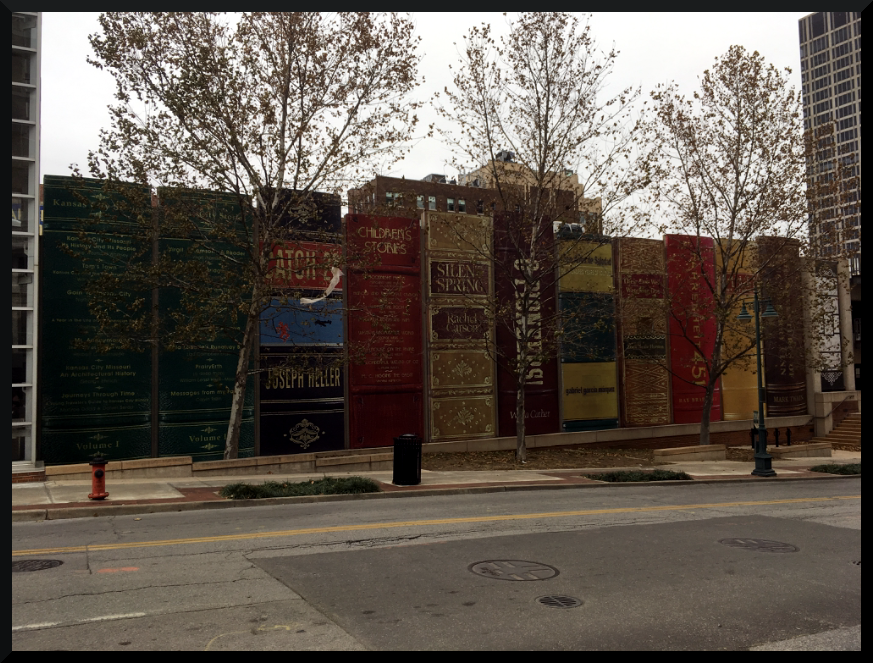
\includegraphics[width=20cm]{./kc_library} % Logo or a photo of you, adjust its dimensions here
\end{minipage}

\vspace{1cm} % A bit of extra whitespace between the header and poster content

%----------------------------------------------------------------------------------------

\begin{multicols}{4} % This is how many columns your poster will be broken into, a poster with many figures may benefit from less columns whereas a text-heavy poster benefits from more

%----------------------------------------------------------------------------------------
%	ABSTRACT
%----------------------------------------------------------------------------------------

%\color{Navy} % Navy color for the abstract
%
%\begin{abstract}
%
%\begin{center}
%\begin{tabular}{ l l }
%
%\hline
%Customer & Con-Met Canton\\
%Part Name & Rear Shelf Outer\\
%Part Number & 69094-000\\
%Shrink & 1.009\\
%Mold Weight & \\
%Mold Size & x, y, z \\
%\hline
%\end{tabular}
%\end{center}
%
%\end{abstract}

%----------------------------------------------------------------------------------------
%	New Work Feasibility Studies 
%----------------------------------------------------------------------------------------

\color{SaddleBrown} % SaddleBrown color for the introduction

\section*{Engineering}
\subsection*{Feasibility}
\begin{enumerate}
\item Consult Part Print and Record Information
	\begin{enumerate}
	\item Part Name
	\item Molding Material
	\item Texture / Finish Specifications
	\end{enumerate}
\item Translate the Customer's part data into NX and Record Information:
	\begin{enumerate}
	\item Part Filename
	\item Current Date
	\item Excerpt from translation log (e.g., solids created, modeling errors, etc.)
	\end{enumerate}
\item In NX, translate the part into die-draw around origin and Record Information:
	\begin{enumerate}
	\item Part Extents
	\item Part Volume
	\item Part Surface Area
	\item Minimum, Maximum and Average Wallstock
	\end{enumerate}
\item Perform Draft Analysis and Record Information:
	\begin{enumerate}
	\item Identify Vertical and Backdrafted Surfaces
	\item Identify Surfaces with less than 3$^\circ$ draft.
	\item Identify Surfaces with less than 1$^\circ$ draft.
	\end{enumerate}
\item Identify and Document Actions---e.g., slides, lifters, etc.
\item Identify and Document Non-Standard Components---e.g., sleeves, cores, inserts, etc.
\item Identify and Document rib depth, tip and root widths.
\item Calculate and Document Steel Sizes.
\end{enumerate}

\subsection*{TKO Data}

\par
\Tree [.S This [.VP [.V is ] \qroof{a simple tree}.NP ] ]
\bigskip

Nulla in nibh mauris. Donec vel ligula nisi, a lacinia arcu. Sed mi dui, malesuada vel consectetur et, egestas porta nisi. Sed eleifend pharetra dolor, et dapibus est vulputate eu. \textbf{Integer faucibus elementum felis vitae fringilla.} In hac habitasse platea dictumst. Duis tristique rutrum nisl, nec vulputate elit porta ut. Donec sodales sollicitudin turpis sed convallis. Etiam mauris ligula, blandit adipiscing condimentum eu, dapibus pellentesque risus.

\subsection*{Preliminary Approval}

%\begin{nd}
%  \hypo {1} {\forall y \neg P(y)}
%  \open
%  \hypo {2} {\exists x P(x)}
%  \open[u]
%  \hypo {3} {P(u)}
%  \have {4} {\forall y \neg P(y)}  \r{1}
%  \have {5} {\neg P(u)}            \Ae{4}
%  \have {6} {\bot}                 \ne{3,5}
%  \close
%  \have {6a}{\bot}                 \Ee{2,3-6}
%  \close
%  \have {7} {\neg \exists x P(x)}  \ni{2-6a}
%\end{nd}

\subsection*{Final Approval}

\textit{Aliquam auctor}, metus id ultrices porta, risus enim cursus sapien, quis iaculis sapien tortor sed odio. Mauris ante orci, euismod vitae tincidunt eu, porta ut neque. Aenean sapien est, viverra vel lacinia nec, venenatis eu nulla. Maecenas ut nunc nibh, et tempus libero. Aenean vitae risus ante. Pellentesque condimentum dui. Etiam sagittis purus non tellus tempor volutpat. Donec et dui non massa tristique adipiscing.

Phasellus imperdiet, tortor vitae congue bibendum, felis enim sagittis lorem, et volutpat ante orci sagittis mi. Morbi rutrum laoreet semper. Morbi accumsan enim nec tortor consectetur non commodo nisi sollicitudin. Proin sollicitudin. Pellentesque eget orci eros. Fusce ultricies, tellus et pellentesque fringilla, ante massa luctus libero, quis tristique \textbf{purus urna nec nibh}.

%----------------------------------------------------------------------------------------
%	OBJECTIVES
%----------------------------------------------------------------------------------------

\color{DarkSlateGray} % DarkSlateGray color for the rest of the content

\section*{Manufacturing}

\begin{enumerate}
\item Lorem ipsum dolor sit amet, consectetur.
\item Nullam at mi nisl. Vestibulum est purus, ultricies cursus volutpat sit amet, vestibulum eu.
\item Praesent tortor libero, vulputate quis elementum a, iaculis.
\item Phasellus a quam mauris, non varius mauris. Fusce tristique, enim tempor varius porta, elit purus commodo velit, pretium mattis ligula nisl nec ante.
\item Ut adipiscing accumsan sapien, sit amet pretium.
\item Estibulum est purus, ultricies cursus volutpat
\item Nullam at mi nisl. Vestibulum est purus, ultricies cursus volutpat sit amet, vestibulum eu.
\item Praesent tortor libero, vulputate quis elementum a, iaculis.
\end{enumerate}

%----------------------------------------------------------------------------------------
%	MATERIALS AND METHODS
%----------------------------------------------------------------------------------------

\section*{Materials and Methods}

Fusce magna risus, molestie ut porttitor in, consectetur sed mi. Vestibulum ante ipsum primis in faucibus orci luctus et ultrices posuere cubilia Curae; Pellentesque consectetur blandit pellentesque. Sed odio justo, viverra nec porttitor vel, lacinia a nunc. Suspendisse pulvinar euismod arcu, sit amet accumsan enim fermentum quis. In id mauris ut dui feugiat egestas. Vestibulum ac turpis lacinia nisl commodo sagittis eget sit amet sapien. Phasellus imperdiet, tortor vitae congue bibendum, felis enim sagittis lorem, et volutpat ante orci sagittis mi. Morbi rutrum laoreet semper. Morbi accumsan enim nec tortor consectetur non commodo nisi sollicitudin. Proin sollicitudin. Pellentesque eget orci eros. Fusce ultricies, tellus et pellentesque fringilla, ante massa luctus libero, quis tristique purus urna nec nibh. Proin sollicitudin. Pellentesque eget orci eros. Fusce ultricies, tellus et pellentesque fringilla, ante massa luctus libero, quis tristique purus urna nec nibh.

%------------------------------------------------

\subsection*{Mathematical Section}

Nulla vel nisl sed mauris auctor mollis non sed. 

\begin{equation}
E = mc^{2}
\label{eqn:Einstein}
\end{equation}

Curabitur mi sem, pulvinar quis aliquam rutrum. (1) edf (2)
, $\Omega=[-1,1]^3$, maecenas leo est, ornare at. $z=-1$ edf $z=1$ sed interdum felis dapibus sem. $x$ set $y$ ytruem. 
Turpis $j$ amet accumsan enim $y$-lacina; 
ref $k$-viverra nec porttitor $x$-lacina. 

Vestibulum ac diam a odio tempus congue. Vivamus id enim nisi:

\begin{eqnarray}
\cos\bar{\phi}_k Q_{j,k+1,t} + Q_{j,k+1,x}+\frac{\sin^2\bar{\phi}_k}{T\cos\bar{\phi}_k} Q_{j,k+1} &=&\nonumber\\ 
-\cos\phi_k Q_{j,k,t} + Q_{j,k,x}-\frac{\sin^2\phi_k}{T\cos\phi_k} Q_{j,k}\label{edgek}
\end{eqnarray}
and
\begin{eqnarray}
\cos\bar{\phi}_j Q_{j+1,k,t} + Q_{j+1,k,y}+\frac{\sin^2\bar{\phi}_j}{T\cos\bar{\phi}_j} Q_{j+1,k}&=&\nonumber \\
-\cos\phi_j Q_{j,k,t} + Q_{j,k,y}-\frac{\sin^2\phi_j}{T\cos\phi_j} Q_{j,k}.\label{edgej}
\end{eqnarray} 

Nulla sed arcu arcu. Duis et ante gravida orci venenatis tincidunt. Fusce vitae lacinia metus. Pellentesque habitant morbi. $\mathbf{A}\underline{\xi}=\underline{\beta}$ Vim $\underline{\xi}$ enum nidi $3(P+2)^{2}$ lacina. Id feugain $\mathbf{A}$ nun quis; magno. Fusce convallis rutrum turpis, quis aliquet enim accumsan id. Vestibulum ullamcorper porttitor convallis. Integer sagittis interdum malesuada. Class aptent taciti sociosqu ad litora torquent per conubia nostra, per inceptos himenaeos. Sed adipiscing tristique orci at ullamcorper. Morbi accumsan, urna et porttitor pulvinar, lacus risus dignissim massa. Proin sollicitudin. Pellentesque eget orci eros. Fusce ultricies, tellus et pellentesque fringilla, ante massa luctus libero, quis tristique purus urna nec nibh.

%----------------------------------------------------------------------------------------
%	RESULTS 
%----------------------------------------------------------------------------------------

\section*{Results}

Donec faucibus purus at tortor egestas eu fermentum dolor facilisis. Maecenas tempor dui eu neque fringilla rutrum. Mauris \emph{lobortis} nisl accumsan. Aenean vitae risus ante. Pellentesque condimentum dui. Etiam sagittis purus non tellus tempor volutpat. Donec et dui non massa tristique adipiscing.
%
\begin{wraptable}{l}{12cm} % Left or right alignment is specified in the first bracket, the width of the table is in the second
\begin{tabular}{l l l}
\toprule
\textbf{Treatments} & \textbf{Response 1} & \textbf{Response 2}\\
\midrule
Treatment 1 & 0.0003262 & 0.562 \\
Treatment 2 & 0.0015681 & 0.910 \\
Treatment 3 & 0.0009271 & 0.296 \\
\bottomrule
\end{tabular}
\captionof{table}{\color{Green} Table caption}
\end{wraptable}
%
Phasellus imperdiet, tortor vitae congue bibendum, felis enim sagittis lorem, et volutpat ante orci sagittis mi. Morbi rutrum laoreet semper. Morbi accumsan enim nec tortor consectetur non commodo nisi sollicitudin. Proin sollicitudin. Pellentesque eget orci eros. Fusce ultricies, tellus et pellentesque fringilla, ante massa luctus libero, quis tristique purus urna nec nibh.

Nulla ut porttitor enim. Suspendisse venenatis dui eget eros gravida tempor. Mauris feugiat elit et augue placerat ultrices. Morbi accumsan enim nec tortor consectetur non commodo. Pellentesque condimentum dui. Etiam sagittis purus non tellus tempor volutpat. Donec et dui non massa tristique adipiscing. Quisque vestibulum eros eu. Phasellus imperdiet, tortor vitae congue bibendum, felis enim sagittis lorem, et volutpat ante orci sagittis mi. Morbi rutrum laoreet semper. Morbi accumsan enim nec tortor consectetur non commodo nisi sollicitudin.

\begin{center}\vspace{1cm}

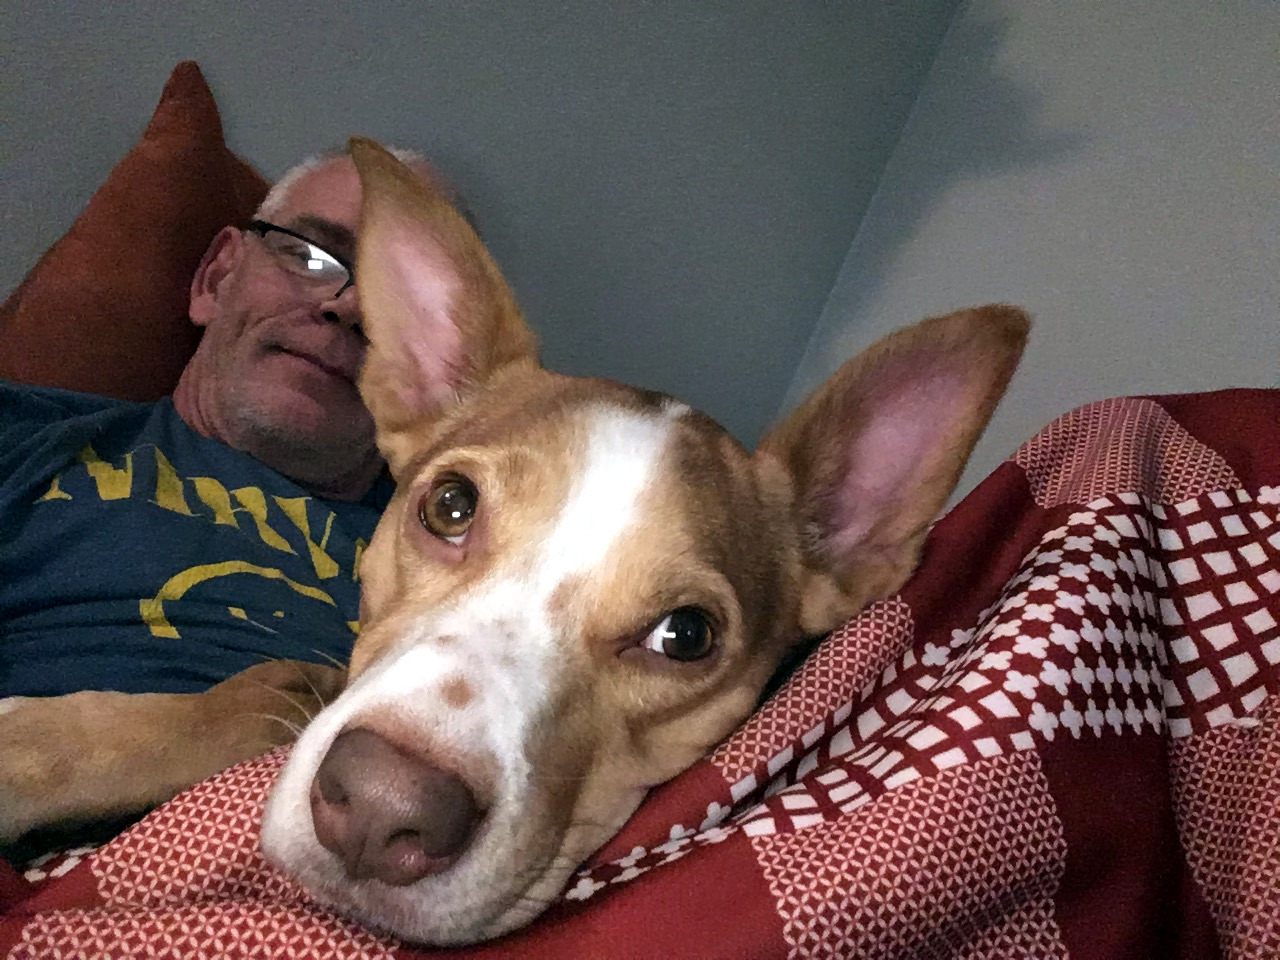
\includegraphics[width=0.8\linewidth]{jake_n_craig.jpg}

\captionof{figure}{\color{Green} Figure caption}

\end{center}\vspace{1cm}

In hac habitasse platea dictumst. Etiam placerat, risus ac.

Adipiscing lectus in magna blandit:

\begin{center}\vspace{1cm}
\begin{tabular}{l l l l}
\toprule
\textbf{Treatments} & \textbf{Response 1} & \textbf{Response 2} \\
\midrule
Treatment 1 & 0.0003262 & 0.562 \\
Treatment 2 & 0.0015681 & 0.910 \\
Treatment 3 & 0.0009271 & 0.296 \\
\bottomrule
\end{tabular}
\captionof{table}{\color{Green} Table caption}
\end{center}\vspace{1cm}

Vivamus sed nibh ac metus tristique tristique a vitae ante. Sed lobortis mi ut arcu fringilla et adipiscing ligula rutrum. Aenean turpis velit, placerat eget tincidunt nec, ornare in nisl. In placerat.

\begin{center}\vspace{1cm}
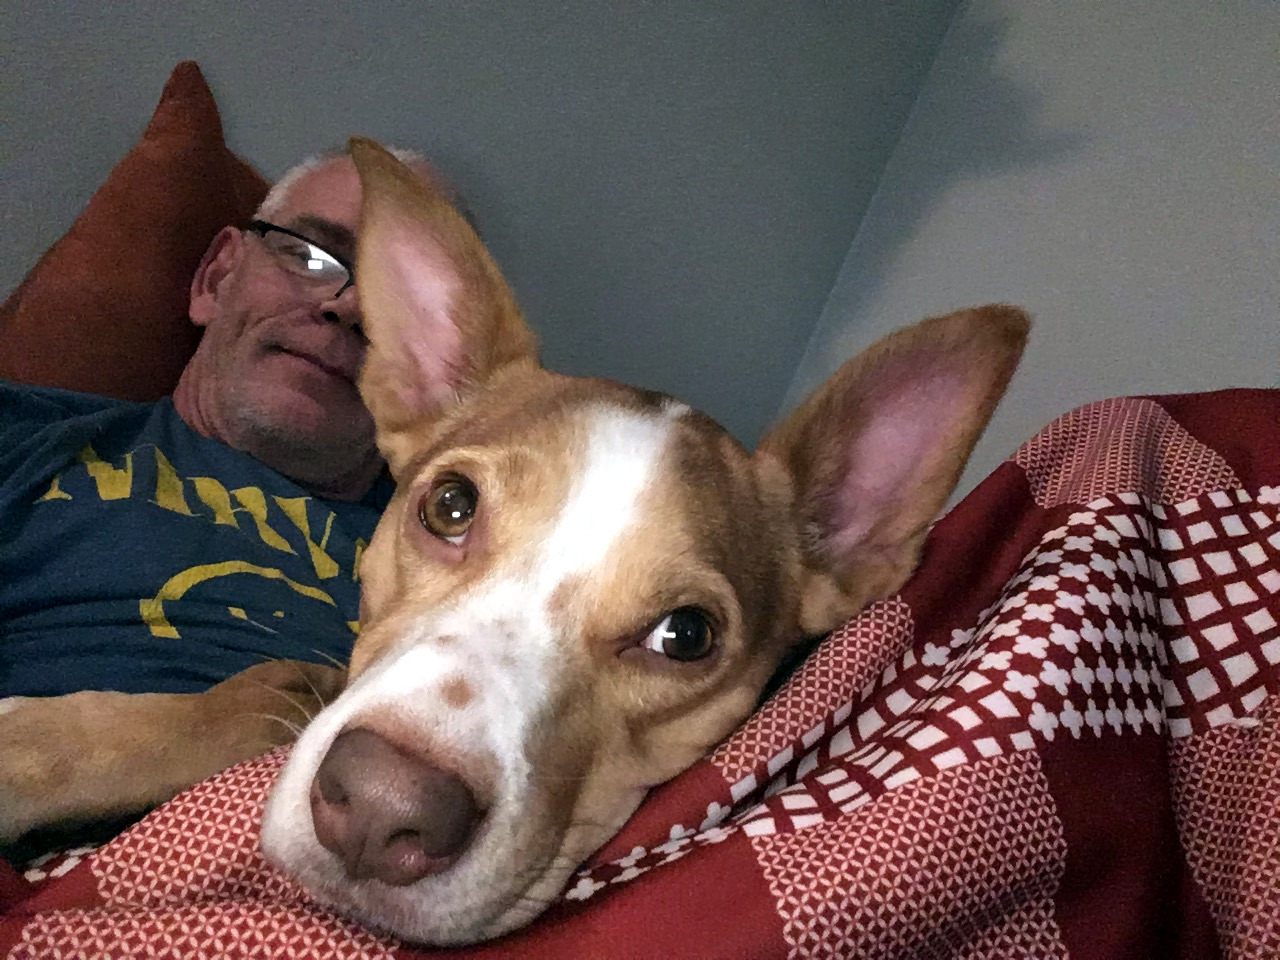
\includegraphics[width=0.8\linewidth]{jake_n_craig.jpg}
\captionof{figure}{\color{Green} Figure caption}
\end{center}\vspace{1cm}

%----------------------------------------------------------------------------------------
%	CONCLUSIONS
%----------------------------------------------------------------------------------------

\color{SaddleBrown} % SaddleBrown color for the conclusions to make them stand out

\section*{Conclusions}

\begin{itemize}
\item Pellentesque eget orci eros. Fusce ultricies, tellus et pellentesque fringilla, ante massa luctus libero, quis tristique purus urna nec nibh. Phasellus fermentum rutrum elementum. Nam quis justo lectus.
\item Vestibulum sem ante, hendrerit a gravida ac, blandit quis magna.
\item Donec sem metus, facilisis at condimentum eget, vehicula ut massa. Morbi consequat, diam sed convallis tincidunt, arcu nunc.
\item Nunc at convallis urna. isus ante. Pellentesque condimentum dui. Etiam sagittis purus non tellus tempor volutpat. Donec et dui non massa tristique adipiscing.
\end{itemize}

\color{DarkSlateGray} % Set the color back to DarkSlateGray for the rest of the content

%----------------------------------------------------------------------------------------
%	FORTHCOMING RESEARCH
%----------------------------------------------------------------------------------------

\section*{Forthcoming Research}

Vivamus molestie, risus tempor vehicula mattis, libero arcu volutpat purus, sed blandit sem nibh eget turpis. Maecenas rutrum dui blandit lorem vulputate gravida. Praesent venenatis mi vel lorem tempor at varius diam sagittis. Nam eu leo id turpis interdum luctus a sed augue. Nam tellus.

 %----------------------------------------------------------------------------------------
%	REFERENCES
%----------------------------------------------------------------------------------------

\nocite{*} % Print all references regardless of whether they were cited in the poster or not
\bibliographystyle{plain} % Plain referencing style
\bibliography{sample} % Use the example bibliography file sample.bib

%----------------------------------------------------------------------------------------
%	ACKNOWLEDGEMENTS
%----------------------------------------------------------------------------------------

\section*{Acknowledgements}

Etiam fermentum, arcu ut gravida fringilla, dolor arcu laoreet justo, ut imperdiet urna arcu a arcu. Donec nec ante a dui tempus consectetur. Cras nisi turpis, dapibus sit amet mattis sed, laoreet.

%----------------------------------------------------------------------------------------

\end{multicols}
\end{document}